% Serial vs orchestrated — before/after. Left (rose): one conversation works
% file-by-file and its context floods. Right (green): a /workflows script fans out
% to workers and only the report returns, so the window stays clean.
% Warm-Tol palette; coordinator=plum, workers=blue, report=green, before=rose.
\documentclass[tikz,border=4mm]{standalone}
\usepackage{tikz}
\usetikzlibrary{positioning, arrows.meta, calc}

\definecolor{warmblue}{HTML}{3B6FA0}
\definecolor{warmrose}{HTML}{C06858}
\definecolor{warmgreen}{HTML}{4A7E3F}
\definecolor{warmplum}{HTML}{8A4E82}

\begin{document}
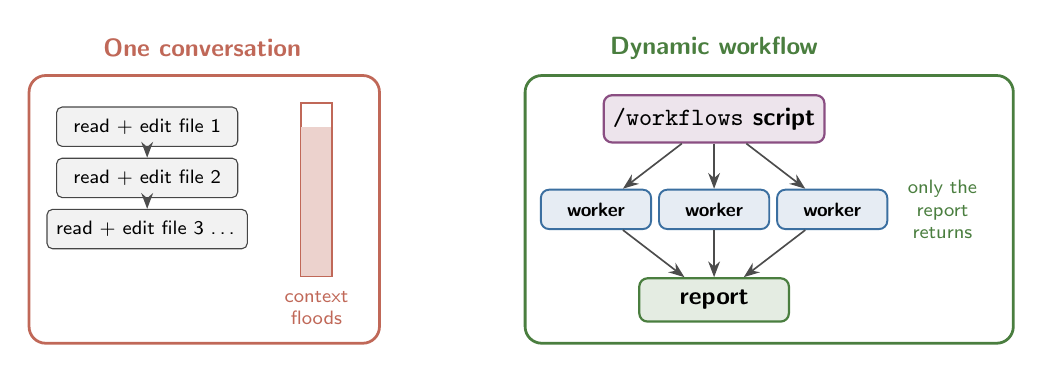
\begin{tikzpicture}[
  font=\sffamily,
  seqstep/.style={draw=gray!55!black, fill=gray!10, rounded corners=2pt,
    minimum width=2.3cm, minimum height=0.5cm, font=\sffamily\scriptsize},
  worker/.style={draw=warmblue, fill=warmblue!13, rounded corners=3pt,
    minimum width=1.4cm, minimum height=0.5cm, font=\sffamily\scriptsize\bfseries, line width=0.7pt},
  coord/.style={draw=warmplum, fill=warmplum!15, rounded corners=3pt,
    minimum width=2.6cm, minimum height=0.6cm, font=\sffamily\small\bfseries, line width=0.8pt},
  report/.style={draw=warmgreen, fill=warmgreen!15, rounded corners=3pt,
    minimum width=1.9cm, minimum height=0.55cm, font=\sffamily\small\bfseries, line width=0.8pt},
  arrow/.style={-Stealth, semithick, draw=gray!60!black},
  ptitle/.style={font=\sffamily\small\bfseries},
  caplabel/.style={font=\sffamily\scriptsize},
]

% ---- LEFT: one conversation, context floods ----
\node[seqstep] (s1) at (0,1.05) {read + edit file 1};
\node[seqstep] (s2) at (0,0.4) {read + edit file 2};
\node[seqstep] (s3) at (0,-0.25) {read + edit file 3 \dots};
\draw[arrow] (s1) -- (s2);
\draw[arrow] (s2) -- (s3);
\draw[draw=warmrose, line width=0.8pt] (1.95,-0.85) rectangle (2.35,1.35);
\fill[warmrose!30] (1.96,-0.84) rectangle (2.34,1.05);
\node[caplabel, text=warmrose, align=center] at (2.15,-1.25) {context\\floods};
\draw[rounded corners=6pt, draw=warmrose, line width=1pt] (-1.5,-1.7) rectangle (2.95,1.7);
\node[ptitle, text=warmrose] at (0.7,2.05) {One conversation};

% ---- RIGHT: dynamic workflow ----
\node[coord] (wf) at (7.2,1.15) {\texttt{/workflows} script};
\node[worker] (w1) at (5.7,0.0) {worker};
\node[worker] (w2) at (7.2,0.0) {worker};
\node[worker] (w3) at (8.7,0.0) {worker};
\draw[arrow] (wf) -- (w1);
\draw[arrow] (wf) -- (w2);
\draw[arrow] (wf) -- (w3);
\node[report] (rep) at (7.2,-1.15) {report};
\draw[arrow] (w1) -- (rep);
\draw[arrow] (w2) -- (rep);
\draw[arrow] (w3) -- (rep);
\node[caplabel, text=warmgreen, align=center] at (10.1,0.0) {only the\\report\\returns};
\draw[rounded corners=6pt, draw=warmgreen, line width=1pt] (4.8,-1.7) rectangle (11.0,1.7);
\node[ptitle, text=warmgreen] at (7.2,2.05) {Dynamic workflow};

\end{tikzpicture}
\end{document}
